\chapter{Contexte}
\label{chap:premierchapitre}

\section{SNCF \& VSCT}
\subsection{Groupe SNCF}
La Société nationale des chemins de fer français (SNCF) est l'entreprise ferroviaire publique française, officiellement créée le 1er janvier 1938 en application du décret-loi du 31 août 1937. Elle est notamment présente dans les domaines du transport de voyageurs, du transport de marchandises et réalise la gestion, l'exploitation et la maintenance du réseau ferré national dont elle est propriétaire.

La SNCF est composée de trois EPIC, mais elle possède de nombreuses filiales aussi bien de droit public que de droit privé qui forment le groupe SNCF.

\subsection{LE GROUPE VSC \& Rail Europe}
VSC Technologie / Voyages-sncf(oui.sncf) / SNCF

Le Groupe VSC et Rail Europe, filiale du Groupe SNCF, dirigée par Franck Gervais, est un acteur majeur du tourisme, expert de la distribution du train mais aussi de la vente des billets d'avions, de séjours, location de voitures et chambres d'hôtel, en France et en Europe. En 2015, son volume d’affaires atteint 4,1 milliards d’euros, en recul de 1,4\% par rapport à 2015 en vendant 86 millions de voyages, en croissance de 4,4\%. L’innovation demeure un axe central et exprime la capacité de Voyages-sncf.com à répondre aux nouveaux usages de ses clients. Aujourd’hui, en France, Voyages-sncf.com est le premier site d’e-commerce et la première agence de voyages en ligne ; le groupe rassemble 1200 collaborateurs dans le monde dont 40\% à l'international (130 en Europe et 350 hors Europe).

En 2000, le site internet Voyages-sncf.com est lancé sur le périmètre France. L’entreprise est à l’époque le distributeur unique des billets de train SNCF, et a pour objectif de transformer son site en portail de voyages offrant des produits et services complémentaires au train. L’année suivante, Voyages-sncf.com forme une joint-venture avec l’américain Expedia et devient une agence de voyage globale. L’entreprise poursuit alors son développement en France, tout en nourrissant une ambition internationale.

Pour répondre aux enjeux de la distribution du voyage et aux nouveaux comportements d’achats, le groupe VSC offre à ses clients mondiaux un réseau puissant, souple et adapté à leurs besoins. Il couvre plus présent dans 11 pays européens et 45 dans le reste du monde via un total de 67 sites internet et mobiles, 4 boutiques et un service de call-center. Afin de répondre aux enjeux spécifiques du marché B2B, le site Voyages-sncf.eu a été lancé en Europe en 12 langues (hors France).
Le site recense plusieurs transporteurs tels que SNCF, TER, Eurostar, Thalys, TGV Lyria ; 3 compagnies de bus, 400 compagnies aériennes ; 280 000 hôtels référencés ; plus de 25 000 offres de séjours ; 30 loueurs de voitures, etc.
\clearpage

\section{Usine Logicielle \& Katana} (à quoi ça sert NDL)
\subsection{Usine Logicielle}
\href{https://wiki.vsct.fr/pages/viewpage.action?spaceKey=KTN\&title=Usine+Logicielle+VSCT}{Usine Logicielle}
L'usine logicielle est l'ensemble de logiciels, d'outils et de procédures qui permettent de structurer et d'industrialiser les développements VSCT, ainsi que leur validation et déploiement sur l'infrastructure VSCT (hors VSCloud).

Dans sa définition actuelle: elle est la continuation de la Nouvelle usine logicielle Lille, et de Katana.

\begin{figure}[h]
\centering
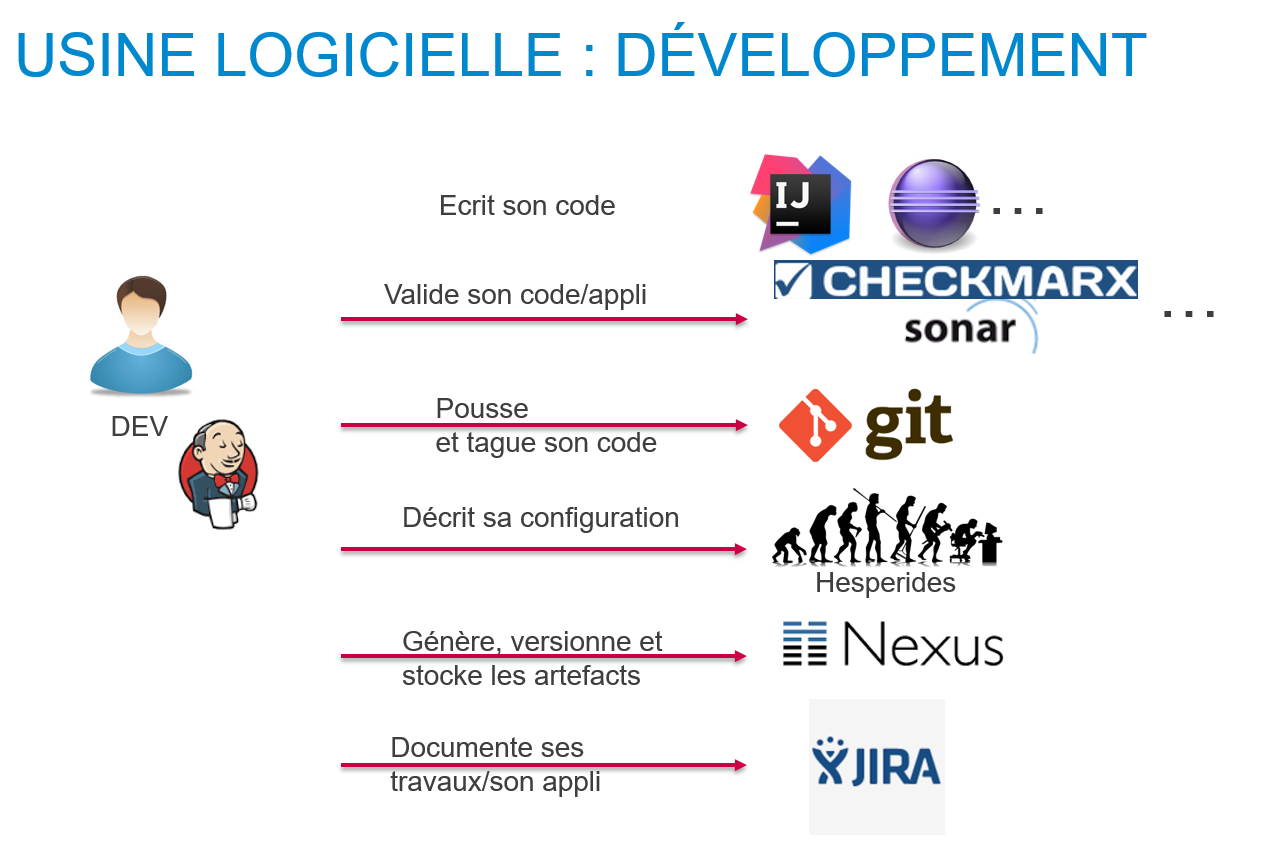
\includegraphics[width=0.8\textwidth]{usine-logicielle-developpement}
\caption{Usine Logicielle: Développement}
\end{figure}

Le développeur édite ses sources sur son poste de travail et les versionne sous GIT, avec entreposage dans une forge GITLAB .

L'application fait elle-même l'objet de versions formalisées, avec les livrables individuels packagés et archivés sur un entrepôt de binaires ( NEXUS ).

Pour chaque application, plusieurs plateformes sont montées sur l'infrastructure pour installer l'application.

Chaque plateforme a un rôle défini. Les plateformes de production font l'objet d'une gestion spécifique, le plus souvent pilotée par les équipes d'exploitation.

Le développeur dispose d'un outillage d'intégration/déploiement continue ( JENKINS ) pour piloter les compilations/générations, validations, déploiements sur des plateforme intermédiaires...
Pour certaines de ces étapes, JENKINS pilote des outils-tiers ( FISHEYE , CRUCIBLE , CHECKMARX , SONAR , ...).

Les serveurs (virtuels ou non) des plateformes sont accessibles en ligne de commande SSH au travers d'un frontal WALLIX, en fonction des droits de chacun.

Un frontal web ( RUNDECK ) permet de mettre à disposition des utilisateurs des opérations de plus haut-niveau, en self-service web sur les serveurs/plateformes (ex: déploiement applicatif, reconfiguration applicative, arrêt/relance et autres opérations spécifiques sur les serveurs).

La configuration détaillée des différentes plateformes de l'application est industrialisée par:
\begin{itemize}
  \item l'outil PUPPET (configuration technique - COTS) et un REFERENTIEL TECHNIQUE en infra-as-code
  \item l'outil HESPERIDES (configuration application - développement VSCT en open-source)
\end{itemize}

Sauf cas particulier, l'accès aux outils et aux plateformes se fait selon l'authentification Active Directory de l'utilisateur.
\subsection{Katana}

\href{https://wiki.vsct.fr/display/KTN/KATANA+Accueil}{Katana}
La solution Katana assure la configuration technique, le déploiement applicatif et autre tâches industrialisées sur les machines des infrastructures VSC(T) de Lille/St-Denis (DMZs hors-production, Assemblage, Perf, Partenaires, Rithmics, Technique, Production, SNB....), à l'exception notable des SIs du CNIT, de VSCloud, et des infra bigData....

\begin{figure}[h]
\centering
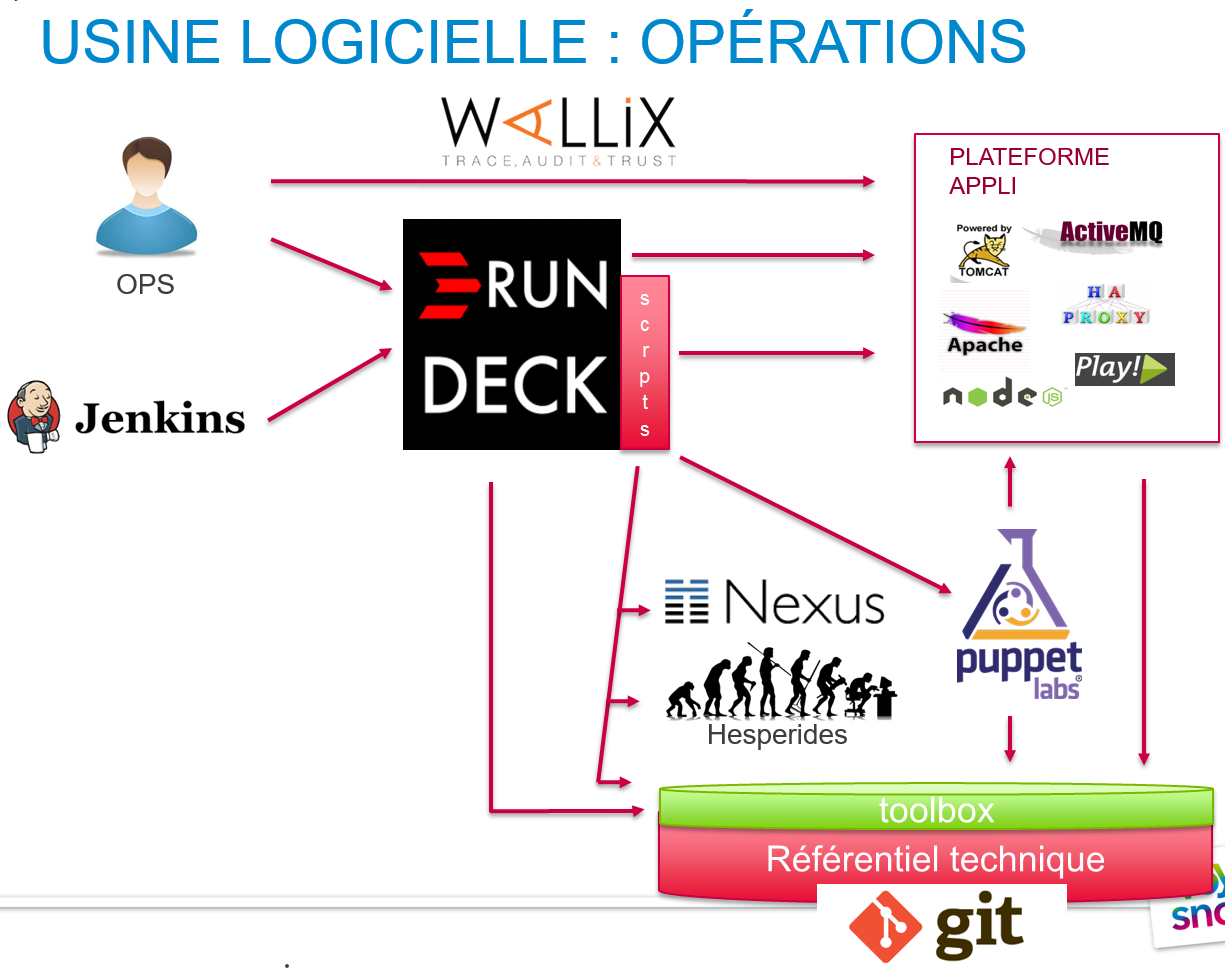
\includegraphics[width=0.8\textwidth]{usine-logicielle-operation}
\caption{Usine Logicielle: Opération}
\end{figure}

Elle est composée :
\begin{itemize}
  \item D'un référentiel de données techniques sur les plateformes/machines sous forme infraAsCode (fichiers envYyaml pour les plateformes, fichiers de configuration Puppet)
  \item D'un référentiel des configurations applicatives: Hesperides (géré par sa propre communauté)
  \item D'un catalogue de scripts (bash/perl/groovy/...), issu des projets de déploiement VSCT, implantant les opérations de déploiement/contrôle/supervision/etc
  \item D'un orchestrateur de tâches en self-service, Rundeck, qui pilote les tâches du Puppet et du catalogue de script (en central, ou sur les machines) .Il peut être contrôlé soit manuellement (par son IHM web), soit par API REST.
\end{itemize}

Katana s'inscrit dans la Usine Logicielle VSCT. La solution s'intègre en particulier avec les outils:
\begin{itemize}
  \item Jenkins: peut piloter l'orchestrateur de tâches dans le cadre des processus d'intégration ou de déploiement continus
  \item Nexus: pour le stockage des livrables applicatifs et autres artefacts (en particulier la note de livraison, le catalogue de scripts, les projets rundeck....)
  \item GIT: pour le stockage et le versionnement des fichiers (code du catalogue de scripts, référentiels de données enYaml, fichiers de configuration Puppet, ...)
\end{itemize}
